\subsection{Vista}

La vista contiene los componentes para representar la interfaz del usuario (IU) del programa y las herramientas con las cuales el usuario puede interactuar con los datos de la aplicación. Adicionalmente, la vista se encarga de recibir e interpretar adecuadamente los datos obtenidos del modelo. Cabe mencionar, que al igual que el resto de componentes del MVC, la clase View implementa la interfaz \say{Notify}, la cual permite la comunicación con el resto de elementos.\bigskip

\texttt{loadContent} es el encargado de cargar el contenido inicial en la ventana. Para esta práctica, carga los siguientes elementos semánticos:\bigskip

\texttt{menu}, función que crea y configura el menú de utilidades de la ventana principal. En esta, se incluyen las siguientes opciones: Abrir ventanas de estadísticas, abrir \say{Word Guesser} y salir del programa.\bigskip

\texttt{body}, función que crea, configura y actualiza la selección de diccionarios. Se trata de una serie de botones que permiten al usuario seleccionar los diccionarios a comparar entre ellos. Además de, una vez ejecutado el algoritmo se permitan visualizar los resultados de forma gráfica.\bigskip

\texttt{sidebar}, función que crea y configura la barra de opciones de la derecha de la interfaz principal. Esta permite al usuario interactuar y configurar el entorno de ejecución de los algoritmos y seleccionar el número de palabras a seleccionar aleatoriamente de cada diccionario. Además, se ha añadido una pequeña ventana de logs para saber que está ocurriendo en todo momento.\bigskip

\texttt{footer}, función que crea y configura los botones para iniciar el algoritmo, además de unos botones para cambiar el \say{Body} a los resultados de la ejecución del algoritmo.

Adicionalmente, a la vista principal, esta permite desplegar una serie de ventanas extra. Una ventana muestra, a tiempo real, el uso y consumo de la memoria de la Java virtual machine (JVM), la otra ventana muestra las estadísticas de la ejecución de los algoritmos además de su comparación, una para abrir el Adivinador de palabras (\ref{Word Guesser}) y un manual de usuario (\ref{Manual usuario, Header}).\bigskip

Finalmente, al ser un módulo de nuestro MVC, implementa la interfaz \texttt{Notify} y su método \texttt{notifyRequest} que le permite recibir notificaciones de los otros módulos del MVC.

\subsubsection{Adivinador de palabras}\label{Word Guesser}

Este apartado de la vista principal, es el encargado de dada una frase, intentar decir al usuario en que idioma se ha escrito la sentencia.\bigskip

Esta ventana está compuesta de 2 principales partes, la parte central de la ventana, y el \say{footer}. En la parte central, se encuentran los resultados, de la entrada del usuario, en un gráfico de barras, donde, el lenguaje con más similitud de la entrada es resaltado en rojo, mientras que, el resto en azul. En la parte inferior, se encuentra una entrada de texto para que el usuario pueda introducir la oración, y un botón de detectar lenguaje.\bigskip

Cabe mencionar, que aparte de poder reconocer una oración, también es capaz de reconocer una única palabra.

\begin{figure}[!h]
    \centering
    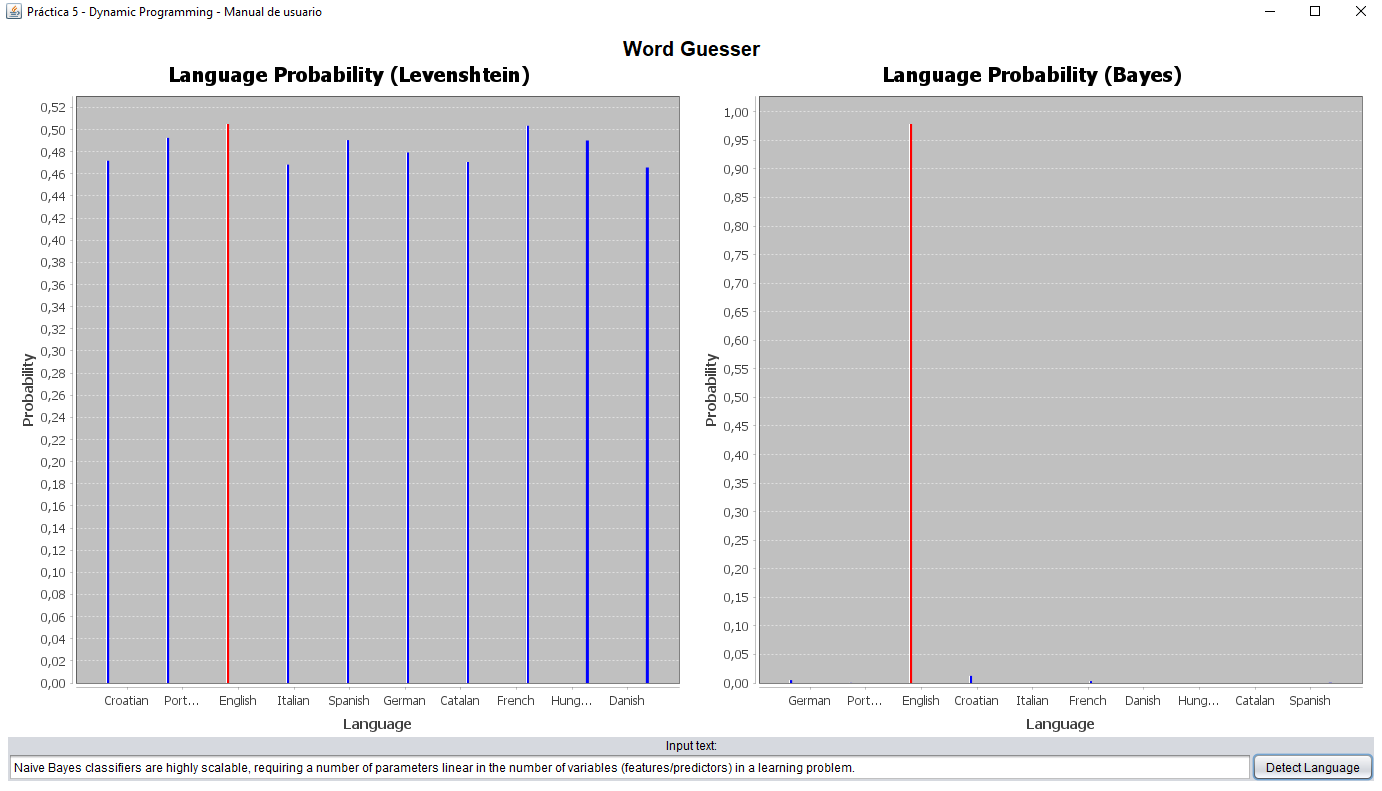
\includegraphics[width=\linewidth]{MVC/View/img/word-guesser.png}
    \caption{Interfaz Word Guesser}
    \label{fig:Ejemplo Word Guesser}
\end{figure}

En el apartado \ref{Word Guesser expl} se explica con detalle la implementación interna del algoritmo para averiguar de qué lenguaje se trata la entrada del usuario.

\subsubsection{Estadísticas JVM}\label{Stats JVM}

Este apartado de la vista principal, es el encargado de enseñar a tiempo real las estadísticas de la máquina virtual de java. Concretamente, se actualiza cada 0.5 s a partir de los datos obtenidos de la clase de java \say{Runtime} y muestra la memoria libre, la memoria total y el uso de esta en una gráfica de líneas, donde el eje x es instante en el tiempo que se han obtenido los datos y el eje y su valor. Todos los datos de la memoria obtenidos están en MB.

\begin{figure}[!h]
    \centering
    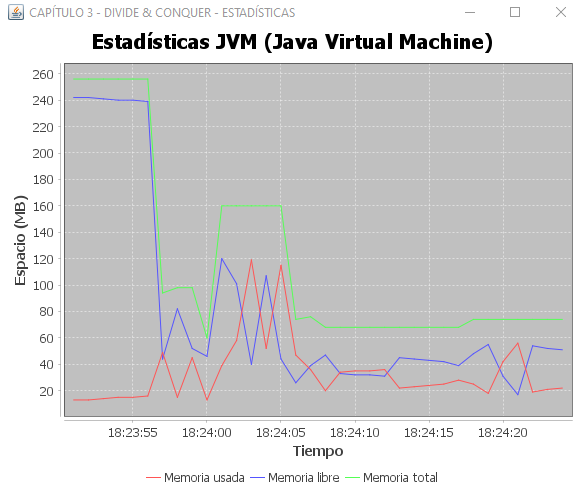
\includegraphics[width=\linewidth]{MVC/View/img/stats-jvm.png}
    \caption{Interfaz estadística JVM}
    \label{fig:Ejemplo stats JVM}
\end{figure}

\subsubsection{Estadísticas de los Algoritmos}\label{Stats Algt}

Este apartado de la vista principal, es el encargado de enseñar las estadísticas de la ejecución de los algoritmos, Levenhstein paralelizado y Levenhstein secuencial. Estas estadísticas incluyen una gráfica con el tiempo de ejecución de cada ejecución del algoritmo. Los resultados (tiempos de ejecución) son representados en un gráfico de barras, donde el eje \textit{x} representa el número de ejecución del algoritmo y el eje y el tiempo en milisegundos que ha tardado.

\begin{figure}[!h]
    \centering
    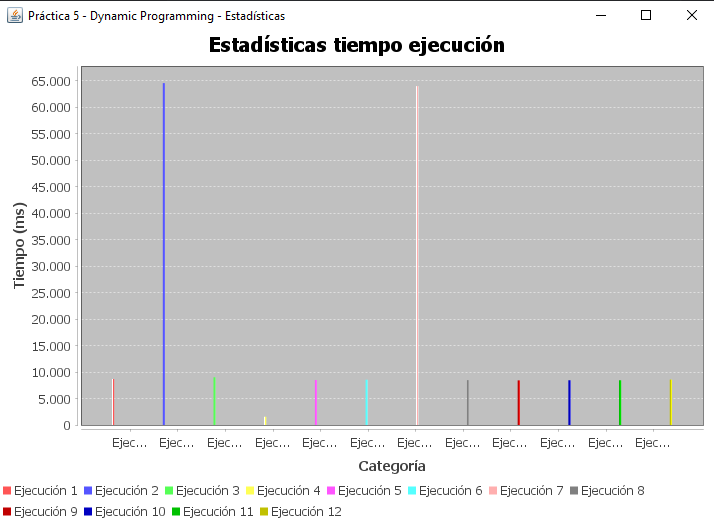
\includegraphics[width=\linewidth]{MVC/View/img/stats-algt.png}
    \caption{Interfaz estadísticas algortimos}
    \label{fig:Ejemplo stats Algt}
\end{figure}

Como se ha podido ver anteriormente en la imagen (\ref{fig:Ejemplo stats Algt}), los datos de las estadísticas están representados con un diagrama de barras, donde el eje x es la categoría a la que pertenecen y el eje y el valor correspondiente.
